\section{Abgrenzung zu Grid Computing}
Der Ansatz -- die Infrastruktur, Rechenleistung sowie Anwendungen oder Speicherplatz über ein Netzwerk für verschiedene Zwecke zur Verfügung zu stellen -- ist kein neuer.
Diese Idee, oder zumindest eine ähnliche, entstand schon vor mehreren Jahren mit dem Begriff \textbf{Grid Computing}.

Im folgenden Abschnitt werden einige Aspekte erläutert, die den Unterschied zwischen Cloud Computing und Grid Computing verdeutlichen.
 
\subsection{Der Begriff \glqq Grid Computing\grqq}
In \cite{grid-checklist} schlägt der Autor eine 3-Punkte-Checkliste vor, anhand deren sich ein Grid-System identifizieren lässt. Demnach ist Grid ein System, das:
\begin{enumerate}
  \item Ressourcen koordiniert, die keiner zentralisierten Kontrolle unterliegen
  \item dabei offene und allgemeine Standardprotokolle und Schnittstellen verwendet
  \item um nicht-triviale \glqq Quality of Services\grqq{} zu liefern
\end{enumerate}

Cloud Computing überschneidet sich nicht nur mit Grid Computing, es ist in der Tat aus Grid Computing entstanden und bildet dessen Rückgrad auf dem seine Infrastruktur aufbaut\cite{360-degree-compared}.

Das spezielle Problem, das dem Konzept des Grids in Wirklichkeit zugrunde liegt,
ist die koordinierte gemeinsame Nutzung von Ressourcen und das Lösen von Problemen
in einer dynamischen institutionsübergreifenden virtuellen Organisation.
Dabei ist mit \glqq gemeinsamer Nutzung\grqq{} der direkte Zugang zu Computern, Software, Daten und anderen Ressourcen,
die für das Lösen von Problemen in industriellen, wissenschaftlichen und technischen Bereichen benötigt werden, zu verstehen.
Das Teilen der Ressourcen beinhaltet klar definierte Regeln, die notwendigerweise stark kontrolliert werden.
Was geteilt werden kann, wer teilen darf und unter welchen Bedingungen geteilt werden darf ist dabei klar und sorgfältig definiert.
Eine Gruppe von Individuen und/oder Institutionen, die durch solche Regeln definiert sind,
bilden die sogenannten \textbf{Virtuellen Organisationen}.\cite{anatomy-of-grid}

\subsection{Anwendungsbereich}

Hier soll es darum gehen, wo hauptsächlich Grid bzw. Cloud Verwendung findet. Z.B. Grid: forschung, rechenintensive Applicationen; Cloud: kommerzielle Zwecke etc.
Bei Anwendungen von Cloud Computing nicht ins Detail gehen, da es schon ein extra Kapitel gibt.

\subsection{Geschäftsmodell}
Typischerweise ist das Geschäftsmodell der Grids (zumindest im akademischen Bereich) projektorientiert und die Anwender oder die Community hat eine bestimmte Anzahl an Serviceeinheiten, die verbraucht werden können\cite{360-degree-compared}.  
Dieses Konzept wird beispielsweise von XSEDE (Extreme Science and Engineering Discovery Environment) -- einem Anbieter von digitalen Dienstleistungen wie Supercomputern -- verwendet\cite{xsede}.
Wenn eine Institution mit ihren eigenen Ressourcen einem solchen Netzwerk beitritt stellt sie diese zur Nutzung für die Community bereit und kann aber dafür auf die Ressourcen der anderen zugreifen\cite{360-degree-compared}.

\subsection{Architektur}
Die Grid-Netze konzentrieren sich auf die Integration vorhandener Ressourcen mit ihrer Hardware, Betriebssystemen, lokalem Ressourcenmanagement und der Sicherheitsinfrastruktur.
Um die Entdeckung sowie die gemeinsame Nutzung von diesen Ressourcen in den sogenannten \glqq Virtuellen Organisationen\grqq{} zu ermöglichen, stellen Grids eine Menge von Standardprotokollen, Middleware, Toolkits sowie Diensten, die auf diesen Protokollen aufbauen, bereit.
Da Ressourcen von verschiedene administrativen Domänen sein können und somit ihre eigene Verwendungsregeln, andere Hard- oder Softwarekonfiguration haben können, stellt die Interoperabilität und Sicherheit das Hauptanliegen für die Gridinfrastruktur dar.\cite{360-degree-compared}

\begin{figure}[ht]
	\centering
  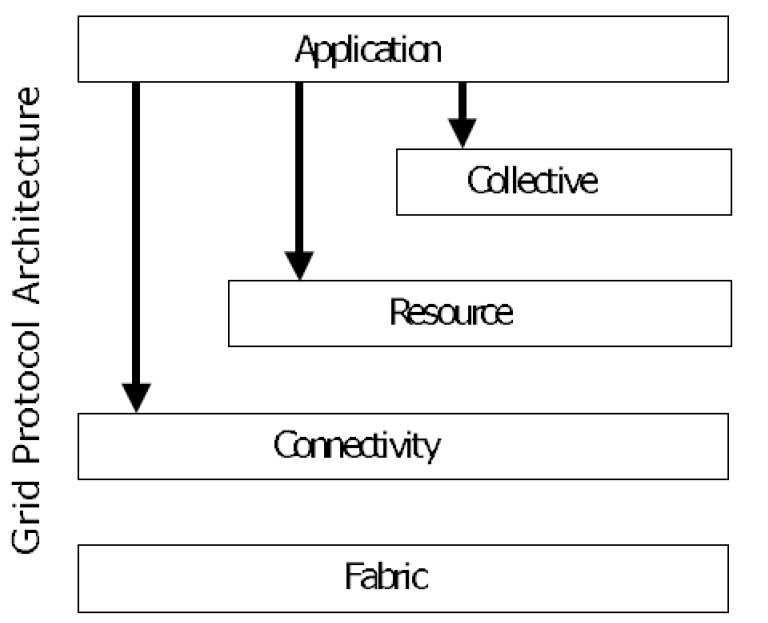
\includegraphics[width=0.5\textwidth]{res/grid-protocol-arch.jpg}
	\caption{Grid protocol architecture\cite{360-degree-compared}}
	\label{gpa}
\end{figure}
\hlred{Die Ressourcen einer virtuellen Organisation können geographisch verteilt sein.}\todo{Zitat finden}

\subsection{Ressourcenverwaltung}
Während Grid Computing versucht Ressourcen zu bündeln, die innerhalb unterschiedlicher Organisationen sich befinden, bietet Cloud Computing diese meistens innerhalb einer einzelnen Organisation. Dies vereinfacht unter anderem solche Aspekte wie Sicherheit, Verfügbarkeit und Heterogenität\cite{comp-cloud-grid-cluster-virt}.

Virtualisierung, Compute Model (Batch-scheduled compute model bei Grid vs Cloud etc.) usw.

\subsection{Fazit}
\hlred{Während Cloud Computing hauptsächlich Lösungen für verschiedene webbasierte Businessfälle bietet, wird Grid Computing dagegen mehr in wissenschaftlichen Projekten bei rechenintensiven Aufgaben eingesetzt.
Grid Computing systems are not intended to be used in business purposes. e.i. there is no business model behind it. The users or organisations who want to make use of Grid Computing simply join a VO and start consuming
Aus Benutzersicht werden Ressourcen bei Cloud Computing zentral verwaltet.
Der Benutzer kann, im Web, vom Cloud Provider zur Verfügung gestellte Schnittstelle verwenden,
um Ressourcen bei Bedarf hinzuzufügen oder zu entfernen.
Grid Computing ist in dieser Hinsicht dezentralisiert. 
Die Ressourcen können sich in unterschiedlichen virtuellen Organisationen befinden.} 

[Wie sieht es für die Zukunft aus?]

\hl{Wird man in der Zukunft komplett auf Grid Computing verzichten können und stattdessen auf Cloud Computing Lösungen zugreifen?}
